\documentclass[12pt, a4paper]{article}
\usepackage[utf8]{inputenc}
\usepackage[IL2]{fontenc}
\usepackage[czech]{babel}
\usepackage{graphicx}

\begin{document}
\begin{figure}[h!]
\centering

\includegraphics[bb= 0 0 820 445 , width=75mm]{favlogo.jpg}
\end{figure}

\vspace{5cm}

{\centering
{\huge Automatický řešitel hry Mastermind}\\[1em]
{\large KIV/UZI - 2. semestrální práce}\\[7,5cm]
}

\begin{tabular}{l r}
student: & Radek VAIS\\
os. číslo: & A13B0457P\\
mail: & vaisr@students.zcu.cz\\
datum: & 6.1.2016\\
\end{tabular}

\thispagestyle{empty}
\newpage

%========================================
%========================================
%========================================
%========================================
%========================================
\section{Zadání} %=====================================================================================================

Napište program, který řeší hru Mastermind (počet políček a barev je vstupním parametrem) sofistikovaným způsobem,
 tj. ne prohledáváním všech alternativ\footnote{Prohledáváním všech alternativ chápejme náhodné zkoušení možností, dokud nedosáhneme úspěchu.}. K~dispozici  by  měly být dvě varianty programu; jedna umožní zadávat ohodnocení 
zvenku (ručně), druhá ohodnocuje automaticky podle zadaného vzoru.  

K~realizaci je možné využít některý z~programovacích jazyků C, C++, Java, Prolog nebo jejich kombinaci. 

Hotovou práci odevzdejte v~jediném archivu typu ZIP prostřednictvím elektronické pošty.

%========================================
%========================================
%========================================
%========================================
%========================================
\section{Analýza~úlohy} %============================================================================================

\subsection{Pravidla hry}

Ve hře Mastermind (neboli Logik) jde o~to, uhádnout tajnou kombinaci protivníka. Kombinace je dána rozmístěním různě barevných prvků na pevný počet pozic. Obvyklé parametry hry jsou šest možných barev na čtyřech různých pozicích, ale není to striktně určeno. K~hádání dostává hráč nápovědu v~podobě černých a bílých kolíků (viz obrázek \ref{fig:game}). Každý barevný prvek, který hádající hráč umístil do správné pozice, je ohodnocen černým kolíkem, každý barevný prvek, který se v~zadané tajné kombinaci vyskytuje, ale není v~dané pozici, je ohodnocen kolíkem bílým. Pokud není kombinace hádajícího hráče ohodnocena žádným kolíkem, znamená to, že se v~tajné kombinaci žádná z~použitých barev v~hodnocené kombinaci nevyskytuje. 

Hráči se ve volbě tajné kombinace a jejím hádání střídají. Počet pokusů při hádání jedné tajné kombinace je omezen. Existují dva způsoby vyhodnocení této hry (tedy určení, který z~hráčů byl lepší). První je to, který z~hráčů odhalil více tajných kombinací soupeře během sudého počtu her. Pokud oba hráči odhalí stejný počet tajných kombinací, vítězí hráč, který ke zjištění potřeboval celkový menší počet pokusů. 

\begin{figure}[ht]
\centering
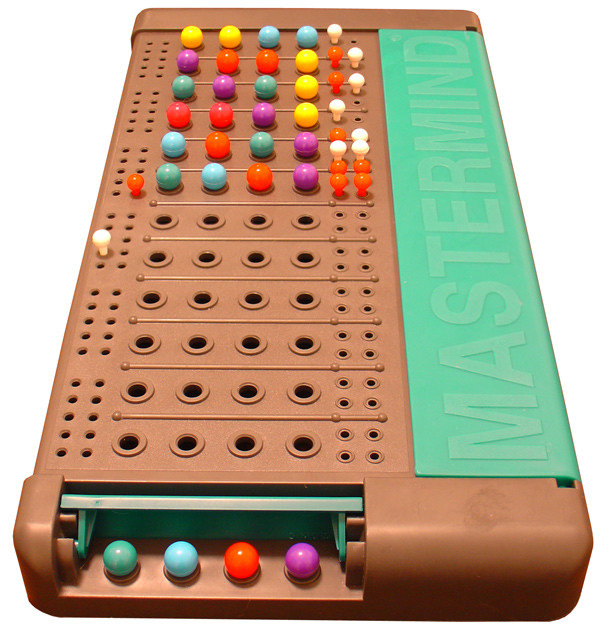
\includegraphics[bb= 0 0 600 637 , height=5cm]{game.jpg}
\caption{Ukázka fyzické hry.}
\label{fig:game}
\end{figure}

Existují dva způsoby hodnocení výhry této hry (který z~hráčů je lepší). Prvním je skutečnost který z~hráčů odhalil více kombinací soupeře během několika her. Pokud, ale oba hráči odhalí všechny kombinace neznáme lepšího. Proto použijeme jako druhý parametr kvality hráče počet tahů, který potřeboval ke zjištění všech kombinací.

\subsection{Metody řešení}

Pro hádání kombinací lze použít různé metody zíkladní přehled poskytuje An Optimal Mastermind (4,7) Strategy and More Results in the Expected Case od Geoffroy \footnote{Geoffroy Ville - Cornell University Library online http://arxiv.org/abs/1305.1010}. Pro bližší rozbor jsem zvolil genetický algoritmus a heuristický algoritmus Donalda Ervina Knutha.

\subsubsection{Genetický algoritmus}

Při tvorbě genetického algoritmu je třeba zvolit vhodné bázové prvky populace, strategii křížení a mutací. Pravděpodobně by toto řešení bylo méně paměťově náročné (oproti Khuthově alg.), pravděpodobně by mělo výrazně pomalejší konvergenci ke správnému řešení. Genetické algoritmy jsou dle mého názoru vhodnější pro případy, kde nepotřebujeme přesný výsledek nýbrž nám stačí kvalitní odhad. 

\subsubsection{Knuthův algoritmus}

Je založený na chytrém výběru řešení z~množiny možných řešení. K~výběru následující kombinace využívá entropii náhodné veličiny, reprezentující ohodnocení konkrétních kombinací vzhledem k~uvažované hádané kombinaci. Vybrána je taková kombinace, jejíž ohodnocení poskytuje maximální střední entropii (viz rovnice \ref{eq:entropy}). Po každém pokusu je dle ohodnocení kombinace protihráčem redukována množina řešení o~všechna, která nevyhovují zadanému ohodnocené. Tento postup se opakuje než zůstane jediné řešení.

\begin{equation}
H(x) = - \sum p(x_i) \cdot log_2(p(x_i))
\label{eq:entropy}
\end{equation}

Existuje několik publikací, které popisují optimalizaci ohodnocovací funkce (výše uvedený výpočet entropie). Výsledky těchto prací ovlivňují rozložení a rozptyl počtu pokusů k~odhalení výsledné kombinace. Viz článek výše. Standardními kritérii pro porovnání různých metod jsou střední počet respektive maximální potřebný pokusů k~odhalení kombinace.

%========================================
%========================================
%========================================
%========================================
%========================================
\section{Popis~implementace} %=======================================================================================

Zvolil jsem implementaci Knuthova algoritmu:
\begin{enumerate}
\item Snaží se minimalizovat počet pokusů ve střední hodnotě.
\item Z~uvedeného článku vyplývá že s~rostoucím počtem barev a pozic se jeho parametry zlepšují.
\item Oproti algoritmům sofistiokvaně pracujícími se stromy se zdá být jednodušší. 
\item Mám zkušenosti s~podobnou úlohou řešenou v~rámci KIV/TI.
\end{enumerate}

\begin{figure}[ht]
\centering
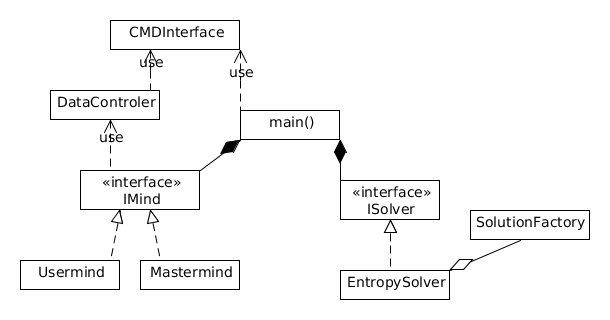
\includegraphics[bb= 0 0 610 320 , width=14cm]{uml.png}
\caption{UML diagram tříd.}
\label{fig:uml}
\end{figure}

K~implementaci jsem zvolil jazyk C++ pro jeho rozšíření o~základní datové struktury (seznamy, mapy, řetězce) oproti jazyku C. Nejedná se o~interpretovaný jazyk, proto od programu očekávám vyšší rychlost provádění oproti interpretovanému jazyku.

Základní stavba programu je znázorněna UML dagramem tříd na obrázku~\ref{fig:uml}. Běh programu je řízen funkcí \texttt{main()}, která zpracuje argumenty a spustí požadované funkce (interaktivní hra, automatická hra, test nebo nápověda). Při vykonávání hlavní funkce pro interaktivní hru \texttt{execGame()} se vytvoří instance tříd IMind a ISolver, které představují instanci hry a instanci řešitele. Poté proběhne cyklus jednoho kola hry (pokusy dokud není skrytá kombinace odhalena). Následně je buď hra ukončena a nebo se spustí opět od inicializace.

Veškerá komunikace s~uživatelem během hry je zprostředkována pomocí třídy \texttt{CMDInterface}. Ke které třídy z~jádra aplikace přistupují pomocí třídy \texttt{DataControler}, která tvoří mezistupeň pro snazší vytvoření grafického uživatelského rozhraní.

\subsection{Rozhraní IMind}
Rozhraní \texttt{IMind} symbolizuje instanci hry. Toto rozhraní deklaruje tuto funkcionalitu:
\begin{verbatim}
 std::vector<bool> trySolution(std::vector<unsigned int> 
                                                 guess_colors)
 bool isSolved()
 unsigned int getPlacesNumber()
 unsigned int getColorNumber()
 void showSolution()
\end{verbatim}
Metoda \texttt{trySolution()} zaručuje získání ohodnocení z~hádané kombinace. V~případě neshody počtu míst pokusu a hádaného řešení je vyhozena výjimka \texttt{WrongCountException()}. Metoda \texttt{isSolved()} informuje, zda byla tajná kombinace odhalena. Metody \texttt{getXX()} slouží k~získání informací o~spuštěné hře. Metoda \texttt{showSolution()} zprostředkuje zobrazení skryté kombinace, při implementaci je kladen důraz na umožněné zobrazení výsledku až po odhalení tajné kombinace.

Toto rozhraní implementují dvě třídy \texttt{Usermind} pro získávání ohodnocení od uživatele a \texttt{Mastermind} pro automatický chod. 

\subsection{Rozhraní ISolver}
Rozhraní \texttt{ISolver} symbolizuje instanci řešitele tajné kombinace. Toto rozhraní deklaruje tuto funkcionalitu:
\begin{verbatim}
std::vector<unsigned int> nextTry()
void getClue(std::vector<bool> clue)
unsigned int numberOfSolutions()
\end{verbatim}

Metoda \texttt{nextTry()} zaručuje získání další hádané kombinace. Metoda \texttt{getClue()} zaručuje předání ohodnocení posledního tahu zpět řešiteli a umožňuje se z~ohodnocení poučit. Metoda \texttt{numberOfSolutions()} slouží k~získání počtu zbývajících řešení, aby bylo možné zjistit, zda ještě řešitel má nějaké odhady v~záloze.

Toto rozhraní implementuje třída \texttt{EntropySolver} která používá výše zmíněný Knuthův algoritmus pro volbu nejvhodnějšího řešení. Ohodnocení tahu je v~aplikaci převedeno na body, za každý přesně určený připočte 10 bodů a za každou barvu na špatném místě 1 bod. S~pomocí takto zjednodušeného ohodnocení se během průchodu metodou \texttt{nextTry()} spočte střední entropie (viz rovnice \ref{eq:entropy}) pro každé nezavržené řešení a řešení s~nejvyšší vrátí jako odhad. Při průchodu metodou \texttt{getClue()} je zmenšen seznam zbývajících ohodnocení na základě předaného ohodnocení. Jsou odstraněna všechna řešení s~jiným bodovým ohodnocením než bylo předáno v~závislosti na posledním odhadu.

%========================================
%========================================
%========================================
%========================================
%========================================
\section{Uživatelská příručka} %======================================================================================

%========================================
%=====================================================================================================================
\subsection{Překlad a~sestavení programu}

Pro automatický překlad pomocí překladače \texttt{gcc}, respektive \texttt{g++} je v~archivu ve složce build připravený soubor Makefile, který slouží k~překladu pomocí programu \texttt{make}. Výstupem je soubor \texttt{Mastermind.exe}. Pokud chcete použít jiný překladač než gcc použijte soubor Makefile pro zjištění vzájemných závislostí modulů\footnote{Další možností je upravit soubor Makefile, zde změnit příkaz překladače, připadně syntaxi příkazů pro překládání, aby odpovídali vašemu překladači.}.

%========================================
%=====================================================================================================================
\subsection{Vstupní data}
Program přijímá vstupní data pomocí argumentů nebo pomocí CLI (uživatelského rozhraní v~konzoli).

%========================================
%=====================================================================================================================
\subsection{Spuštění a~běh programu}

Jedná se o~konzolovou aplikaci, proto spuštění provádíme z~příkazové řádky příkazem \texttt{Mastermind.exe [type [num1 num2]]}. Při spuštění bez parametrů program zahájí interaktivní herní režim a zjistí od uživatele potřebné informace.

\subsubsection{Parametry příkazové řádky}
Jako typ (\texttt{type}) spuštění lze použít \texttt{h} (případně \texttt{?}) bez dalších parametrů. Což vyvolá nápovědu ke spuštění programu. Typ spuštění \texttt{t} vyžaduje další dva parametry počet barev a počet pozic. Spuštění s~tímto parametrem ověří funkčnost generátoru možných řešení. Typ spuštěni \texttt{a} také vyžaduje další dva parametry. Opět jde o~počet barev a počet pozic. Tento parametr spustí variantu programu, která ke svému běhu nepotřebuje interakci uživatele. Pokud zvolíme jinou kombinaci parametrů, bude automaticky spuštěn program v~režimu interaktivní hry.

\begin{table}[htb]
	\centering
	\begin{tabular}{c | c}
		parametry & efekt\\
		\hline
		\texttt{h} & nápověda\\
		\texttt{?} & nápověda\\
		\texttt{t u\_int u\_int} & test generátoru řešení\\
		\texttt{a u\_int u\_int} & automatický režim
	\end{tabular}     

	\caption{Tabulka shrnuje možné argumenty pro spuštění programu.}
	\label{tab:args}
\end{table}

\subsubsection{Interaktivní režim}

Program v~režimu interaktivní hry vykonává smyčku, během které postupně zjistí parametry hry, provede postup řešení a ukončí program nebo spustí nové kolo od zjištění parametrů hry. Během zjišťování parametrů si program vyžádá dvě celá kladná čísla, která znamenají počet možných barev a počet pozic. Třetím parametrem je mechanismus ohodnocení. Tato volba určuje, kdo zadává ohodnocení a tedy si i vymyslí tajnou kombinaci (počítač nebo uživatel). 

Za předpokladu, uživatelského ohodnocení hry je třeba mít na paměti mechanismus zadávání ohodnocení odhadu do počítače. Za každou správnou barvu na správném místě zadejte \texttt{1} a za každou správnou barvu na špatném místě zadejte \texttt{0}. Jednotlivé ohodnocení se zadává po jednom znaku. A~každé místo může být ohodnoceno právě jednou. Pro ukončení ohodnocení zadejte znak \texttt{N}. Pokud provedete ohodnocení chybně, počítač není schopen to rozpoznat ve chvíli vaší chyby a hra pravděpodobně skončí nenalezením správného řešení.  

%========================================
%========================================
%========================================
%========================================
%========================================
\newpage
\section{Závěr}  %======================================================================================================


Vytvořený program byl testován 30 náhodnými úlohami pro 6 barev a 4 pozice, které vyřešil se střední hodnotou 4,60 pokusů a maximálním počtem   6 pokusů. (viz příloha) Vzhledem k~tomu, že pro tento počet barev a pozic existuje celkem 1296 různých kombinací, nelze výše uvedené zjištěné hodnoty porovnávat s~výsledky získanými jinými metodami a uváděnými v~literatuře (viz tabulka \ref{tab:data}). Na vytvoření programu, který automaticky prověří řešení všech kombinací a získá tak relevantní statistické hodnoty, již nezbyl čas, nebylo to ani předmětem zadání.

\begin{table}[ht]
\begin{tabular}{c | c | c}

Algoritmus & Střední počet pokusů  & Maximální počet pokusů\\
\hline
Max. size  	&   4,476 &  5\\
Expect size	 &4,395   & 6\\
Entropy      &  4,416  & 6\\
Most parts   &   4,373 &  6\\
Optimal      &   4.340 &  6\\

\end{tabular}
\label{tab:data}
\caption{Výsledky pro optimalizovaný běh programu z~výše uvedeného článku. Pro konfiguraci 6 barev 4 pozice.}
\end{table}
		

Bylo možné pouze porovnání s~optimálním stromem pro řešení úlohy pro 2 barvy a 3 pozice, který je uváděn v~literatuře. Vytvoření optimálního stromu pro obecný počet barev a pozic ovšem není reálné.

\begin{table}[h]
\centering
\begin{tabular}{c | c }

Kombinace &   Počet pokusů\\
\hline
111  & 3\\
112  & 1\\
121  & 2\\
122  & 2\\
211  & 3\\
212  & 3\\
221  & 2\\
222  & 2\\

\end{tabular}

Střední počet pokusů:  18/8 = 2,25
Maximální počet pokusů:  3 
\caption{Výsledky pro optimální algoritmus.}
\end{table}



\begin{table}[h]
\centering
\begin{tabular}{c | c }

Kombinace &   Počet pokusů\\
\hline
111  & 3\\
112  & 3\\
121  & 2\\
122  & 2\\
211  & 1\\
212  & 3\\
221  & 2\\
222  & 2\\

\end{tabular}

Střední počet pokusů:  18/8 = 2,25
Maximální počet pokusů:  3 
\caption{Výsledky pro implementovaný algoritmus.}
\end{table}

Pro vyšší počty barev a pozic si může implementovaný algoritmus dávat o~něco málo horší výsledky než jsou uváděny v~literatuře (u~dvou barev a třech pozic tento efekt nenastal). Bylo by to dáno tím, že jsem vhodný tah vybíral pouze z~postupně redukované množiny možných řešení, přestože existují situace, kdy některé kombinace, které již nemohou být řešením, přinášejí ve střední hodnotě maximální informaci (ovšem za cenu delší doby výpočtu, která by s~narůstajícím počtem barev a pozic rostla exponenciálně). 

\newpage
\section*{Příloha}  

\begin{table}[ht!]
\centering
\begin{tabular}{c | c }

Kombinace &   Počet pokusů\\
\hline
2513 & 4\\
1664 & 5\\
2612 & 4\\
6633 & 4\\
2413 & 4\\
2163 & 5\\
2566 & 5\\
2161 & 5\\
4535 & 6\\
3614 & 5\\
2136 & 5\\
4231 & 3\\
4645 & 5\\
1511 & 4\\
4541 & 4\\
3536 & 5\\
4234 & 5\\
1651 & 4\\
1242 & 5\\
2245 & 5\\
3415 & 6\\
5266 & 5\\
6144 & 4\\
4326 & 6\\
3524 & 5\\
2546 & 5\\
5231 & 4\\
3254 & 4\\
1351 & 4\\
5114 & 3\\
 

\end{tabular}

\caption{Testovací výsledky pro implementovaný algoritmus a kombinace 6 barev a 4 pozice.}
\end{table}


\end{document}